\subsection{Avaliação de Parsers de Constituência} 
\label{subsec:avaliacao_parsers}
Para verificar se um dado parser é capaz de classificar corretamente novas sentenças dadas, existem algumas métricas desenvolvidas. Dentre as mais conhecidas, se destacam as \textit{PARSEVAL Measures}, e sua derivação, a \textit{F-Measure}.
% Mas vamos falar primeiro sobre medidas clássicas no estudo de NLP estatístico.

% ------------------------------------------------------

\subsubsection{\textit{PRECISION, RECALL, F1-SCORE}}
\label{subsubsec:eval_measures}
Considerando um treinamento supervisionado (como no caso dos nossos \textit{parsers}), temos um conjunto de exemplos corretos (chamados \textit{gold standard}, padrão ouro), que podemos usar para comparar com os resultados obtidos pelo sistema desenvolvido. Considerando o padrão ouro como nosso objetivo/alvo, podemos obter uma tabela semelhante à Tabela \ref{tab:tab_confusao}. Como descrito por \citeonline[p~368]{Manning1999FoundationsNLP},
\begin{quote}
    \textquote{\textit{The cases accounted for by \textit{tp} (true positives) and \textit{tn} (true negatives) are the cases our system got right. The wrongly selected cases in \textit{fp} are called false positives, false acceptances or Type II errors. The cases in \textit{fn} that failed to be selected are called fake negatives, false rejections or Type I errors.}}
    \footnote{\textquote{Os casos considerados \textit{tp} (verdadeiro positivo) e \textit{tn} (verdadeiro negativo) são casos em que nosso sistema acertou. Os casos selecionados erroneamente em \textit{fp} são chamados falso positivos, falsas aceitações, ou erros Tipo II. casos em \textit{fn} que falharam de ser selecionados são chamados falsos negativos, falsas rejeições, ou erros Tipo I}. Tradução própria}
\end{quote}
\begin{center}
    \begin{table}[!h]
    \centering
    \begin{tabular}{c|c c}
                    &       &   Actual\\
        System      & target &  $\neg$target\\
        \hline
        selected    & tp & fp \\
        $\neg$selected   & fn & tn 
    \end{tabular}
    \caption[Tabela de Confusão]{Tabela de Confusão, ou \textit{contingency matrix}. Adaptado de \cite[p~268]{Manning1999FoundationsNLP} }
    \label{tab:tab_confusao}
\end{table}
\end{center}

A partir daí podemos definir duas métricas, \textit{precision} e \textit{recall}\footnote{Precisão e Revocação}. Por \cite[p~268-269]{Manning1999FoundationsNLP} \textit{precision} é definida como a medida da proporção de itens selecionados que o sistema acertou. \textit{Recall} é definida como a medida da proporção dos itens alvo que o sistema selecionou. Podemos ver ambas na equação  \ref{eq:precision_recal}.
\begin{center}
    \begin{equation}
\label{eq:precision_recal}
    precision = \frac{tp}{tp+fp}, 
    \hspace{10mm}
    recall = \frac{tp}{tp+fn}
\end{equation}
\end{center}

A medida F-measure, também conhecido por F1-score \cite[p~262]{derczynski2016complementarity} é, por \cite[p~1]{truthFScore}, a média harmônica entre \textit{precision} (P) e \textit{recall} (R), como pode ser visto na Equação \ref{eq:f_score}. Seus valores variam entre 0 e 1. 
\begin{center}
    \begin{equation}
\label{eq:f_score}
    F = 2P \frac{R}{P + R}
\end{equation}
\end{center}

% ------------------------------------------------------

\subsubsection{\textit{PARSERVAL MEASURES}}
\label{subsubsec:parseval}
As PARSERVAL measures são basicamente três: \textit{precision} (ou \textit{labeled precision}, LP), \textit{recall} (ou \textit{labeled recall}, RB) e \textit{crossing brackets}, que seguem uma lógica semelhante à supracitada em \ref{subsubsec:parseval}. Dado um \textit{parser} que gere uma árvore, \cite[p~433-434]{Manning1999FoundationsNLP}
\begin{quote}
    \textquote{\textit{Precision is how many brackets in the parse match those in the correct tree, recall measures how many of the brackets in the correct tree are in the parse, and crossing brackets gives the average of how many constituents in one tree cross over constituent boundaries in the other tree.}}
    \footnote{\textquote{Precisão é quantos parênteses na árvore gerada combinam com aqueles da árvore correta, revogação mede quantos parênteses na árvore correta estão na árvore gerada, e parênteses cruzados dá a média de quantos constituintes em uma árvore cruza com as fronteiras na outra árvore}. Tradução própria.}
\end{quote}
\begin{center}
    \begin{figure}[!ht]
    \centering
    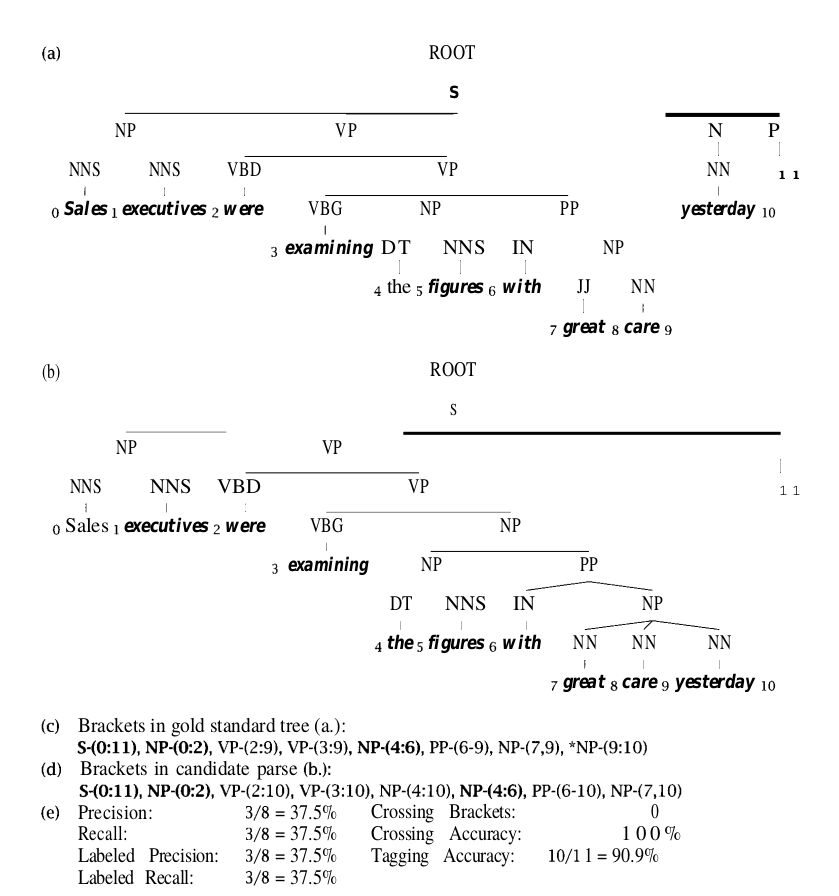
\includegraphics[width=\textwidth]{imagens/fig_demo_parseval.png}
    % \includesvg[width=.8\textwidth]{demo}
    % \includesvg{imagens/cintil_pcfg}
    \caption[Demonstração do funcionamento do PARSERVAL]{Demonstração do funcionamento do PARSERVAL. Extraido de \citeonline[p~433]{Manning1999FoundationsNLP}. Note que o nó NP-(9:10) (\textit{yesterday}), ao ser posicionado como filho do nó NP-(7:10), torna todos os nós acima dele também errados.}
    \label{fig:demo_parseval}
\end{figure}
\end{center}

Nesse contexto, o cálculo do F-MEASURE se dá utilizando a mesma Equação \ref{eq:f_score}.

Algumas críticas podem ser feitas à esse sistema. \citeonline{constParsEvalYT} demonstra que essa medida é muito sensível à propagação de erros em cascata. Ou seja, um constituinte mal colocado num nível mais baixo da árvore faz com que todos os nós acima dela também estejam errados, reduzindo muito a pontuação. \citeonline{parserEvalSecret} também nota que \textquote{\textit{The problem of standard Parseval is that it counts nodes as the same regardless of the underlying structure they dominate}}
\footnote{\textquote{O problema do PARSERVAL padrão é que ele conta nós como os mesmos, independente da estrutura subalterna que estes dominam}. Tradução própria.}.

Isto pode ser melhor observado na Figura \ref{fig:demo_parseval}. Numa sentença $W=[w_0 \ldots w_n]$, para $w_j$ palavras, os nós dá árvore são identificados por $P-(i:f)$, sendo $P$ a \textit{POS tag}, $i$ o inicio da \textit{abrangência} do nó, e $f$ o final. Nós com mesma \textit{POS} são identificados pela ordem de aparecimento na árvore, e pela abrangência. Por \textit{abrangência}, refere-se ao alcance de todos os seus descendentes. Assim, na árvore \ref{fig:demo_parseval}[a], o primeiro VP é representado por $VP-(2:9)$ por englobar a sentença de \textquote{\textit{were}} a \textquote{\textit{care}}. Note que, ao posicionar o último NP, referente à \textquote{\textit{yesterday}}, a árvore candidata o marca como $NP-(7:10)$, em contraste com o \textquote{padrão-ouro}, que deveria ser $NP-(9:10)$. Isto faz com que, não só este nó esteja errado, como todos os nós acima dele, fazendo com que os valores de LP, LR e, por fim, F1 sejam afetados negativamente.